% !TEX root = ../main.tex
\chapter{Introduction}\label{main_introduction}


\section{Motivation}
Segmentation is an important problem in computer vision as a first step
towards understanding an image. Many algorithms start with an over-segmentation
into superpixels.
The superpixel segmentation can be interpreted as a \emph{region adjacency graph} (see \cref{fig:make_rag}) and
well studied graph-theoretical approaches can be applied to analyze and segment such a graph \cite{vlachos_1993_csv}.







%\addtocontents{lof}{%
%    \protect\centerline{%
%      \protect\includegraphics[width=.25\linewidth]{myimage}%
%    }%
%  }%


%\newsavebox{\meinebox}

\begin{figure}
  %\savebox{\meinebox}[30mm][l]{
  \begin{center}
  \subfloat[$3x3$ image]{\label{fig:gg_33}
    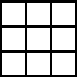
\includegraphics[width=0.15\textwidth]{fig/grid33.pdf}
  }\hspace{1cm}
  \subfloat[4-NH graph]{\label{fig:gg_33_4}
    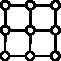
\includegraphics[width=0.15\textwidth]{fig/grid33_4.pdf}
  }\hspace{1cm}
  \subfloat[8-NH graph]{\label{fig:gg_33_8}
    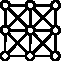
\includegraphics[width=0.15\textwidth]{fig/grid33_8.pdf}
  }
  \end{center}
  %}
  \addtocontents{lof}{%
    \vspace{1cm}
    \protect\centerline{%
      \protect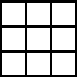
\includegraphics[width=.075\linewidth]{fig/grid33.pdf} \hspace{0.2cm}
      \protect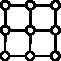
\includegraphics[width=.075\linewidth]{fig/grid33_4.pdf}\hspace{0.2cm}
      \protect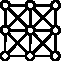
\includegraphics[width=.075\linewidth]{fig/grid33_8.pdf}%
    }%
  }%
  \caption[An image treaded as grid graph]{ \label{fig:grid_graph}
  An image as in \Cref{fig:gg_33} can be interpreted as a grid graph. 
  Two different types of grid graphs can be defined for an image.
  \Cref{fig:gg_33_4} shows a grid graph with 4-neighborhood,
  \cref{fig:gg_33_8}  with 8-neighborhood.  
  }
\end{figure}


%\begin{figure}
%\usebox{\meinebox}
%\caption{
%fubar
%}
%\end{figure}

Many algorithms have been generalized to $n$-dimensional images.
Since a $n$-dimensional image itself can be interpreted as a \emph{grid graph}  (see \cref{fig:grid_graph}) any graph-based algorithm can be applied to images, if they are treated as grid graphs.

Therefore, \emph{graph-based image analysis} can be viewed as a generalization of \emph{image analysis}.
From a theoretical and  point of view, such a generalization is very desirable.
For example, it allows to easy apply well studied graph-theoretical approaches, such as clustering
to  \emph{image analyses} \cite{vlachos_1993_csv,arbelaez_2006_cvpr,ohlander_1978_cgip}.

From an algorithmic point of view, such a generalization can help to reduce 
code redundancy.
Generic graph algorithms can be written once, and might be applied 
to grid graphs (2D, 3D, 3D+t) and irregular graphs ( \eg \quad regions adjacency graphs and nearest neighbor graphs).

In addition, many graph-based algorithms are composed  of
very simple building blocks such
as \emph{minimum spanning trees}, \emph{hierarchical clustering} and 
\emph{shortest path algorithms}. 

Providing generic and reusable implementations of these building blocks
 is therefore beneficial.






\begin{figure}
\centering
\subfloat[$8x8$ image]{ \label{fig:make_rag_grid}
    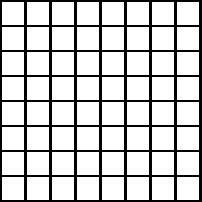
\includegraphics[width=0.25\textwidth]{fig/gridA.pdf}
}
\subfloat[$8x8$ grid graph]{  \label{fig:make_rag_grid_graph}
    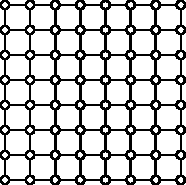
\includegraphics[width=0.25\textwidth]{fig/gridGraphA.pdf}
}
\subfloat[labeled image]{   \label{fig:make_rag_labels_labels}
    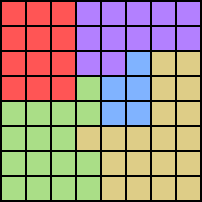
\includegraphics[width=0.25\textwidth]{fig/lgridA.pdf}
}
\\
\subfloat[labeled grid graph]{   \label{fig:make_rag_labels_on_graph}
    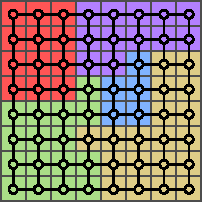
\includegraphics[width=0.25\textwidth]{fig/gridC.pdf}
}
\subfloat[RAG]{     \label{fig:make_rag_rag_a}
    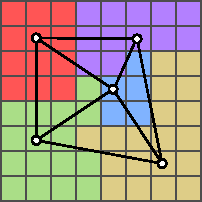
\includegraphics[width=0.25\textwidth]{fig/lgridB.pdf}
}
\subfloat[RAG]{     \label{fig:make_rag_rag_b}
    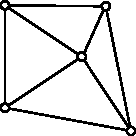
\includegraphics[width=0.25\textwidth]{fig/lgridC.pdf}
}
  \addtocontents{lof}{%
    \vspace{1cm}
    \protect\centerline{%
      \protect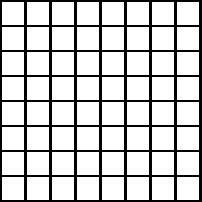
\includegraphics[width=.075\linewidth]{fig/gridA.pdf}  \hspace{0.2cm}
      \protect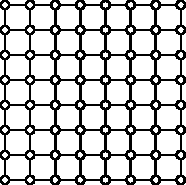
\includegraphics[width=.075\linewidth]{fig/gridGraphA.pdf}\hspace{0.2cm}
      \protect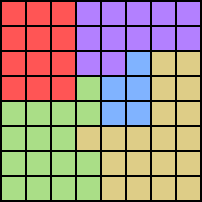
\includegraphics[width=.075\linewidth]{fig/lgridA.pdf} 
    }%
    \vspace{0.2cm}
    \protect\centerline{%
      \protect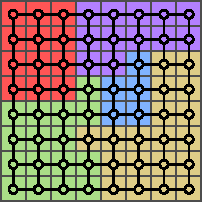
\includegraphics[width=.075\linewidth]{fig/gridC.pdf}  \hspace{0.2cm}
      \protect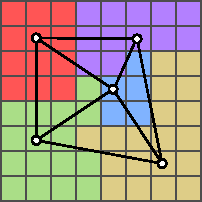
\includegraphics[width=.075\linewidth]{fig/lgridB.pdf}\hspace{0.2cm}
      \protect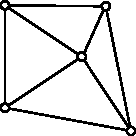
\includegraphics[width=.075\linewidth]{fig/lgridC.pdf}%
    }%
  }%
\caption[Make a region adjacency graph from a labeled graph]{
    A labeled grid graph  (\cref{fig:make_rag_grid}, \cref{fig:make_rag_grid_graph}  and \ref{fig:make_rag_labels_labels})
    or any other graph can be turned into a region adjacency graph (\cref{fig:make_rag_labels_on_graph}, \cref{fig:make_rag_rag_a} and \cref{fig:make_rag_rag_b}). 
    Any edge  $\{u,v\}$ where $u$ and $v$ have the same label is contracted and $u$ and $v$ 
    are merged.
}\label{fig:make_rag}
\end{figure}


\section{Contributions}

Within this thesis we make the following contributions:

\begin{inparaenum}[(i)]
    \item 
    We propose and implement a library for graph-based image analysis 
        implemented within the \emph{VIGRA} library \cite{koethe_2000_phd_thesis,software_vigra}. 
    \item 
        We also provide implementations for important graph-based algorithms based on the proposed library.
        All data structures and algorithm are implemented in fast C++,
    \item but can also be used from Python for rapid prototyping.
    \item Ready to use examples are given within this thesis.




    \item
      A new perspective on solving the multicut problem by
      \emph{local} move making methods together with
      %
      \item
      a new approximate multicut solver called
      \emph{Cut, Glue \& Cut (CGC)}. Furthermore,
      %
      \item our method avoids re-solving the same moves
      by tracking their ``dirtyness'', which decreases the runtime. 
      %
      \item
      An extensive evaluation on existing and new benchmark datasets shows
      that CGC provides results close to optimality
      and equal application performance significantly faster than all its
      competitors, both exact
      and approximative methods, and gives new insights concerning the applicability
      of competing methods.
\end{inparaenum}




\section{Organization}

This work is organized in the following way.
In \cref{ch:reated_work} related work will be presented and  discussed.
In \cref{ch:cgc} we propose a new algorithm for the multicut objective.
In Sec.~\ref{sec:problem_formulation} we review two common formulations
of the multicut problem. 
A detailed related work w.r.t. multicuts is given in \cref{sec:gcg_related_work}.
Based on a general formulation of local partition moves on segmentations in
\cref{sec:cut_moves},
we describe our new Cut, Glue \& Cut algorithm
in \cref{sec:cut_glue_cut_algorithm}. Extensive experiments
on benchmark datasets are presented in \cref{sec:experiments},
where we show an extensive comparison  with existing solvers.

In \cref{ch:vigra_graph_lib} describe our implementation of
a graph-based library build on top of VIGRA \cite{koethe_2000_phd_thesis,software_vigra}. 
The used graph APIs are discussed in \cref{sec:graph_apis}.
The different graph classes implemented within VIGRA
will be presented in \cref{sec:impl_graphs}, where
design choices are discussed and most 
important implementation details are explained.
All design choices related to \emph{Python} will
be discussed separately within \cref{sec:graph_lib_python}.
Ready to use code examples will be given in \cref{ch:the_showcase}.
In \cref{ch:conclusion} the presented is concluded
and future research topics related to this thesis are presented.




